\documentclass{article}
\usepackage{amsmath, amssymb, amsthm, dsfont, physics, hyperref, cleveref}
\usepackage{graphicx}
\usepackage[margin=1.5cm]{geometry}
\usepackage{biblatex}

\title{Screening of airborne radioxenon measurements for Nuclear-Test-Ban Treaty verification}
\author{Jerome Alhage, Jelle Bosmans, Thomas Ceulemans, Nick Dewaele}
\date{}

\newtheorem{proposition}{Proposition}
\newtheorem{remark}[proposition]{Remark}

\addbibresource{library.bib}

\begin{document}
    \maketitle

    \begin{abstract}
        We extend a simulation model for radioxenon emissions by inferring daily emissions of sources in the Northern Hemisphere. This is done by numerical optimisation of the relative prediction error over the daily emissions.
    \end{abstract}

\section{Introduction}
The Comprehensive Nuclear Test Ban Treaty \cite{CTBT} bans all atmospheric, underwater and underground nuclear explosions when it enters into force. Compliance with the Treaty will be verified by the International Monitoring System to which SCK-CEN contributes as a National Data Centre. As part of the monitoring system, more than 300 measuring stations have been set up worldwide including seismic, hydro-acoustic, infrasound and radionuclide detectors. In this paper, we focus on the radionuclide detectors and in particular on measurements of radioactive xenon or \emph{radioxenon} concentrations. Monitoring of radioxenon concentrations is particularly useful for the detection of underground nuclear explosions, since radioxenon readily escapes the explosion zone owning to its properties as a noble gas. However, civilian sources such as medical isotope production facilities and nuclear power plants also emit radioactive xenon and this \emph{civilian background} complicates the detection of nuclear explosions.

One approach under study at SCK-CEN explicitly models the \emph{xenon weather} using emission data from civilian sources and atmospheric transport modelling. If this approach can be used to accurately predict the civilian background, emissions caused by nuclear explosions can be separated from civilian sources. In this paper, we adapt the simulation model of radioxenon emissions and transport developped at SCK-CEN. This model operates on a map of $m = 200$ civilian sources of radioxenon with their average daily emissions $x_1,\dots,x_m$. A list of $n = 4636$ measurements $[y_1,\dots,y_n]$ at stations spread across the Northern Hemisphere is given. The relationship between the emissions and the measured concentrations is given by a linear model,  
\begin{equation}
    \label{eq: initial model}
y_i \approx
\hat{y}_i = \sum_{j=1}^m \sum_{\Delta = 1}^{15}  M_{i,(j,\Delta)} \frac{x_{j}}{s_j}
\end{equation}
where the sensitivities $M_{i,(j, \Delta)}$ are obtained from backward simulation of the atmospheric transport. The scaling factors $s_j$ arise from the simulation on a mesh of the Northern Hemisphere. In particular, they compensate for the fact that not all cells in the mesh have the same volume. 
The \emph{sensitivity matrices} $M_{i,(j,\Delta)}$ can be interpreted as the contribution of the emission from source $j$ from $\Delta$ days before the measurement to the $i$'th concentration measurement in the dataset. The contributions of more than $15$ days before the measurement are neglected. A certain source will only contribute to the measurements that are relatively close to it, depending on the prevailing wind directions that facilitate atmospheric transport. Hence, many sensitivity matrices will contain zeros when there is no transport from the source to the measurement location.

\subsection{Outline}
The above assumes that the xenon emission is constant for every source. We adapt this model in \cref{sec: model} so that daily emissions are taken into account. In \cref{sec: nondetections}, we discuss the use of a transformation from \cite{deMeutter2022uncertainty} to model the accuracy in a non-detection event.
In \cref{sec: optimisation}, we explain a method to fit the extended model to the measured concentration data. Given the time constraints of this project, the optimality criterion was deliberately kept simple. Numerical data in \cref{sec: numerical results} show that the average prediction error can be decreased. We conclude in \cref{sec: further work} with suggestions to make the model more realistic and improve computational aspects.

\subsection{Notation}
\begin{itemize}
    \item $\vb{1}_q = [1\,\, \dots\,\, 1]^T \in \mathbb{R}^q$ is the constant vector consisting of only ones.
    \item $\odot$ is the Hadamard (i.e.\, elementwise) product, given by $(AB)_{ij} = A_{ij} B_{ij}$.
    \item $\mathrm{vec}(\bullet): \mathbb{R}^{p \times q} \rightarrow \mathbb{R}^{pq}$ is the vectorisation operator. It can be understood as stacking the columns of a matrix in one long vector. 
    \item $\mathrm{diag}$ is the canonical identification of $p$-vectors and $p \times p$ diagonal matrices, i.e.,
    $$
    \mathrm{diag}\left(
    \begin{bmatrix}
        a_1 \\ 
        \vdots \\
        a_p
    \end{bmatrix}
    \right)
    =
    \begin{bmatrix}
        a_1 & 0 & \dots & 0 \\
        0 & a_2 & \dots & 0 \\
        \vdots & \vdots & \ddots & 0 \\
        0 & 0 & \cdots & a_p
    \end{bmatrix}
    .$$
    \item $\otimes$ is the Kronecker product. In particular,
        $$
        \underbrace{
        \begin{bmatrix}
            a_1 \\
            \vdots \\
            a_p
        \end{bmatrix}
        }_{\in \mathbb{R}^{p}}
        \otimes 
        \underbrace{
        \begin{bmatrix}
            1 \\
            \vdots \\
            1
        \end{bmatrix}
        }_{\in \mathbb{R}^{q}}
        =
        \underbrace{
        \begin{bmatrix}
            a_1 \\
            \vdots \\
            a_1 \\
            a_2 \\
            \vdots \\
            a_2 \\
            \vdots \\
            a_p
        \end{bmatrix}
        }_{\in \mathbb{R}^{pq}}
        .$$
        A standard rule of thumb in numerical linear algebra is that the Kronecker product serves a mostly theoretical purpose and is rarely calculated explicitly.
        This is because the Kronecker product satisfies $\mathrm{vec} \left(AXB\right) = \left(B^T \otimes A\right) \mathrm{vec}\left(X\right)$ for all matrices $A,X,B$ \cite[eq. 1.3.6]{Golub2013}.
    \item For a vector-valued function $F(x)$, the Jacobian matrix is denoted as $\frac{\partial F}{\partial x}$.
\end{itemize}

\section{Model}
\label{sec: model}

\subsection{Reformulation of the baseline model}

\Cref{eq: initial model} can be formulated as follows:
\begin{align}
    \label{eq: initial model concise} 
\begin{bmatrix}
    \hat{y}_1 \\ 
    \vdots \\
    \hat{y}_{n}
\end{bmatrix}
&=
\begin{bmatrix}
    M_{1,(1,1)} & M_{1,(1,2)} & \cdots & M_{1,(m,15)} \\
    \vdots & \vdots & & \vdots \\
    M_{n,(1,1)} & M_{n,(1,2)} & \cdots & M_{n,(m,15)} \\
\end{bmatrix}
\begin{bmatrix}
    s_1^{-1} x_1\\
    \vdots \\
    s_1^{-1} x_1 \\
    s_2^{-1} x_2 \\
    \vdots \\
    s_n^{-1} x_m
\end{bmatrix} 
\\
&=
\begin{bmatrix}
    M_{1,(1,1)} & M_{1,(1,2)} & \cdots & M_{1,(n,15)} \\
    \vdots & \vdots & & \vdots \\
    M_{m,(1,1)} & M_{m,(1,2)} & \cdots & M_{m,(n,15)} \\
\end{bmatrix}
\left( 
     S^{-1}
     \begin{bmatrix}
        x_1 \\
        \vdots \\
        x_n
     \end{bmatrix}
     \otimes \vb{1}_{15}
\right)
\nonumber
\end{align}
where $S = \mathrm{diag}([s_1,\dots,s_m])$.
In this section, we present a different interpretation. Instead of $S^{-1} x \otimes \vb{1}_{15}$, we make a vector $\tilde{x} := S^{-1} x \otimes \vb{1}_{T}$ where $T = 365 + 15 = 380$. This is a vector of length $mT$ that gives the emission from the most recent day to $T$ days in the past for each source. This is assumed to be constant for all days. Therefore, $\tilde{x}$ consists of $m = 200$ blocks, each of which is a constant vector of length $T$.

We can write a system of equations that is logically the same as \cref{eq: initial model concise} but uses $\tilde{x}$ instead of $S^{-1} x \otimes \vb{1}_{15}$. This gives a larger linear system. Because the emission from most dates has a negligible contribution to the observed concentrations, many coefficients in the larger matrix will be zero. For every measurement $i$, we have the linear relationship
$$
        \hat{y}_i
    =
    \begin{bmatrix}
        \cdots & M_{i,(1,1)} & \dots & M_{i,(1,15)} & 0 & \dots & M_{i,(2,1)} & \dots & M_{i,(2,15)} & \dots
    \end{bmatrix}
    \tilde{x}
.$$
The presence of zeros in the matrix indicates that emissions from the distant past do not contribute to the observed concentrations. Furthermore, recall many of the sensitivity matrices themselves also contain zeros. Hence the larger matrix has a sparse nature.

Assume for the sake of simplicity that in each station, there is one observation per day, indexed as $y_{k,t}$, where $k = 1,\dots,K$ where $K$ is the number of stations and $t = 1,\dots,365$. The index $t=1$ corresponds to the most recent measurement. Then the full system reads as follows:
\begin{equation}
    \label{eq: initial model 365 days}
\begin{bmatrix}
    \hat{y}_{1,1} \\
    \hat{y}_{1,2} \\
    \vdots \\
    \hat{y}_{2,1} \\ 
    \vdots \\
    \hat{y}_{K,365}
\end{bmatrix}
=
\underbrace{
\begin{bmatrix}
    M_{(1,1), (1,1)} & M_{(1,1), (1,2)} & \cdots & M_{(1,1),(1,15)} & 0 & \cdots & \cdots & M_{(1,1), (2,1)} & \cdots & 0 \\
    0 & M_{(1,2), (1,1)} & \cdots & M_{(1,2), (1,14)} & M_{(1,2), (1,15)} & 0 & \cdots & 0 & \cdots & 0 \\
    \vdots & \vdots & & \vdots & \vdots & \vdots & & \vdots & & \vdots \\
    M_{(2,1), (1,1)} & M_{(2,1), (1,2)} & \cdots & M_{(2,1),(1,15)} & 0 & \cdots & \cdots & M_{(2,1), (2,1)} & \cdots & 0 \\
    \vdots \\
    \vdots
\end{bmatrix}
}_{ := M_{shift}}
\tilde{x}
.\end{equation}

\begin{remark}
    As an alternative to using $\tilde{x} = S^{-1} x \otimes \vb{1}_T$, one could use the permuted expression $\vb{1}_{T} \otimes (S^{-1} x)$. This is a vector containing all emissions on day 1, followed by all emissions on day 2, etc. A similar permutation of $y$ could be chosen. These permutations can be compensated by the inverse permutation on the columns and rows of $M_{shift}$, respectively. The resulting model is essentially identical to \cref{eq: initial model 365 days} but may have advantages when it comes to implementation in software. We will not consider this.
\end{remark}

\subsection{Model with time-dependent correction to the emissions}
Daily emissions can be modelled by multiplying the average emission of source $j$ by some scaling factor $w_{j,t}$. This corresponds to the 
transformation
$$
\begin{bmatrix}
    s_1^{-1} x_1 \\
    \vdots \\
    s_1^{-1} x_1 \\ 
    s_2^{-1} x_2 \\
    \vdots \\ 
    s_m^{-1} x_m
\end{bmatrix}
\mapsto
\begin{bmatrix}
    w_{1,1} s_1^{-1} x_1 \\
    \vdots \\
    w_{1,T} s_1^{-1} x_1 \\ 
    w_{2,1} s_2^{-1} x_2 \\
    \vdots \\ 
    w_{m, T} s_m^{-1} x_m
\end{bmatrix}
$$
which can be written concisely as $W\tilde{x}$ where $W = \mathrm{diag}([w_{1,1}, w_{1,2},\dots,w_{m,T}])$.
Using this weighted vector of emissions instead of $\tilde{x}$ in \cref{eq: initial model 365 days} gives
\begin{equation}
    \label{eq: time-evolving model concise}
\hat{y} = M_{shift} W \tilde{x}
.\end{equation}
In the next section, we present a method to fit the unknown factors $W$ to the data.

\section{Correction for non-detections}
\label{sec: nondetections}

Sometimes, the concentration at a measurement station is below the minimum detectable concentration (MDC). The corresponding measurements are $y_i = 0$.
To account for non-detections, we apply the transformation $h$ from \cite{deMeutter2022uncertainty}. This is given by the continuously differentiable function
$$
h(y) = \begin{cases}
    \frac{y^2}{4MDC} + MDC &\quad \text{if } y \le 2MDC \\
    y &\quad \text{else}
\end{cases}
.$$
This transformation maps the interval $[0, MDC]$ onto $[MDC, 2MDC]$. For observations that are significantly larger than $MDC$, this is approximately the identity. If $y$ and the simulated value $\hat{y}$ are both larger than $2MDC$, then $h(\hat{y}) / h(y) = \hat{y} / y$. If $y = 0$ because the concentration is not detectable, then we want a simulated value $\hat{y}$ such that $h(\hat{y}) \approx MDC$. In both cases, we can use the value of $h(\hat{y}) / h(y)$ as an indication of the accuracy of the simulation.


In the dataset that we are working with, we know the values of $- \frac{M_{i,(j,\Delta)}}{MDC}$ for every non-detection event. In these events, we work as if $MDC = 1$. If the predicted value is $\hat{y}_i < 0$, we have 
$$
h\left(\hat{y}\right) = \begin{cases}
    \frac{\hat{y}^2}{4} + 1 &\quad\text{if } \hat{y} \le -2 \\
    -\hat{y} &\quad\text{else}
\end{cases}
$$
and $h(y) = 1$. For the detection events, we do not have the $MDC$ and cannot calculate $h$ exactly. For the detection events, we can approximate $h$ by the identity map.

\section{Fitting the model}
\label{sec: optimisation}

In the above, we argued that the prediction is accurate if $h(\hat{y})$ is close to one, where $\hat{y}$ is the predicted concentration. This is equivalent to $\log^2(h(\hat{y}))$ being small. Notice that this penalises overestimates by a factor $\alpha$ as much as underestimates by a factor $\alpha$. That is, 
$$
\log^2(\alpha) = \log^2(\alpha^{-1})
.$$
The average prediction error over all predictions is $\sum_{i=1}^n \log^2(h(\hat{y}_i)) = \norm{\log h.(\hat{y})}^2$, where $\log h.$ is the elementwise application of $x \mapsto \log h(x)$. This will be the first criterion for optimality of the model.

The second criterion is the ratio between the daily emissions and the average emission for each source, i.e. the factors $W$. In a similar vein as the above, the size of $W$ can be measured as $\norm{\log W}^2$ where $\norm{\cdot}$ is the Frobenius norm\footnote{Since $W$ is a diagonal matrix, the matrix logarithm $\log W$ is simply the diagonal matrix with $\log w_{1,1}, \log w_{1,2}, \dots$ on the diagonal. Hence, $\norm{\log W}^2 = \log^2 w_{1,1} + \log^2 w_{1,2} + \dots$}. 

To balance these two criteria, we measure the quality of the model as 
\begin{equation}
    \label{eq: cost function regularised}
f(W) := 
\underbrace{\frac{1}{2}\norm{\log h.(\hat{y}(W))}^2}_{\text{prediction error}} + \underbrace{\frac{1}{2}\lambda \norm{\log W}^2}_{\text{deviation from average emission}}
\quad\text{where}\quad 
\hat{y}(W) = M_{shift} W \tilde{x}
\end{equation}
where $\lambda \ge 0$ is a regularisation parameter.

Observe that the model where $W$ is the identity matrix $\mathds{I}$ is equivalent to the original model. Furthermore, the regularisation term vanishes if and only if $W = \mathds{I}$. That is,
$$
f(\mathds{I}) = \frac{1}{2}\norm{\log h.(\hat{y}(\mathds{I}))}^2
$$
is the prediction error for the original model.
For $W \ne \mathds{I}$, the regularisation term is strictly positive. This means that, if $f(W) \le f(\mathds{I})$, then the prediction error is decreased, i.e.,
$$
\frac{1}{2}\norm{\log h.(\hat{y}(W))}^2
\le
\frac{1}{2}\norm{\log h.(\hat{y}(\mathds{I}))}^2
.$$
Hence, the model corresponding to the minimum of \cref{eq: cost function regularised} predicts the data at least as accurately as the original model.

To optimise $f$ numerically, we will parametrise $W$ in \cref{eq: cost function regularised} as $W = e^{\mathrm{diag}\, v}$ where $v = [v_1, v_2,\dots]$ is some vector and $e^{\mathrm{diag}\, v}$ is the diagonal matrix with $[e^{v_1}, e^{v_2},\dots]$ on the diagonal. The motivation for doing this is twofold:
\begin{enumerate}
    \item It ensures that $W$ remains strictly positive. In particular, the diagonal elements of $W$ can only tend towards zero if $v_j \rightarrow -\infty$ for some $i$. 
    \item It implicitly measures changes to $W$ in a relative sense. If the optimisation algorithm performs a linear update $v_{k+1} = v_k + \Delta v$, this corresponds to a relative update $W_{k+1} = W_k e^{\mathrm{diag}\, \Delta v}$.
\end{enumerate}

Thus, in practice, we are interested in the optimisation problem
\begin{equation}
    \label{eq: cost function parameterised}
\min_{v} f(v)
\quad\text{where}\quad 
f(v)
=
\frac{1}{2}\norm{\log h.(\hat{y})}^2 + \frac{1}{2}\lambda \norm{v}^2
\quad\text{and}\quad 
\hat{y} = M_{shift} e^{\mathrm{diag}\, v} \tilde{x}
.\end{equation}

Most optimisation algorithms require at least the gradient of $f$. This is given by the following:
\begin{proposition}
    Let $g = [g_1, \dots, g_n]$ be the vector defined elementwise by 
    $$
    g_i = \frac{\log h(\hat{y}_i)}{h(\hat{y}_i)} \frac{\mathrm{d}}{\mathrm{d}\hat{y}_i} h(\hat{y}_i)
    .$$
    Then 
    $$
    \mathrm{grad}\, f(v) = e^v \odot (M_{shift}^T g) \odot \tilde{x} 
    $$
    where $e^v$ denotes elementwise exponentiation and $\odot$ is the Hadamard (elementwise) product.
\end{proposition}
\begin{proof}
Let $W = e^{\mathrm{diag}\, v}$ and let $U$ be the matrix corresponding to the linear map $\mathrm{vec} \circ \mathrm{diag}$. Then $\mathrm{vec}\left(W(v)\right) = U e^v$.
Define $$
F(v) := \log h.(\hat{y}(v))
.$$
By using basic properties of the Kronecker product \cite[eq. 1.3.6]{Golub2013}, we have
$$
\hat{y}(v) = M_{shift} W(v) \tilde{x}
=
(\tilde{x}^T \otimes M_{shift}) \mathrm{vec} \left(W(v)\right)
=
(\tilde{x}^T \otimes M_{shift}) U e^v
,$$
so that
$$
\frac{\partial F}{\partial v}
=
\underbrace{\mathrm{diag}\left(
    \left.\frac{\mathrm{d}}{\mathrm{d}x} \log h(x)\right\vert_{x = \hat{y}(v)}
    \right)}_{:= H}
\frac{\partial \hat{y}}{\partial v}
=
H (\tilde{x}^T \otimes M_{shift}) U e^{\mathrm{diag}\, v}
.$$
The matrix $H$ appearing in this expression is defined by the diagonal elements 
$$
H_{ii} = \frac{1}{h(\hat{y}_i)}\left(\left.\frac{\mathrm{d}}{\mathrm{d}x} h(x)\right\vert_{x = \hat{y}_i} \right)
.$$
Using standard differentiation rules for the squared norm of a vector-valued function, we obtain
\begin{align*}
\mathrm{grad}_v\, \left(\frac{1}{2} \norm{F(v)}^2 \right)
&=
\left(\frac{\partial F}{\partial v}\right)^T F(v) \\
&= e^{\mathrm{diag}\, v} U^T (\tilde{x} \otimes M_{shift}^T) H \log h.(\hat{y}) \\
&= e^{\mathrm{diag}\, v} U^T (\tilde{x} \otimes M_{shift}^T) g \\
&= e^{\mathrm{diag}\, v} U^T \mathrm{vec}\left(M_{shift}^T g \tilde{x}^T\right)
\end{align*}
Since $U$ is the unitary map that maps a vector onto (the vectorisation of) the corresponding diagonal matrix, $U^T$ maps the vectorisation of a matrix onto its diagonal.
Since the diagonal of the rank-1 matrix $M_{shift}^T g \tilde{x}^T$ is $(M_{shift}^T g) \odot \tilde{x}$, the above simplifies to
$$
\mathrm{grad}_v\, \left(\frac{1}{2} \norm{F(v)}^2 \right)
=
e^{\mathrm{diag}\, v} \left( (M_{shift}^T g) \odot \tilde{x} \right) = e^{v} \odot (M_{shift}^T g) \odot \tilde{x}
.$$


The foregoing gives the derivative of the first term in the definition of $f(v)$. The gradient of the second term is simply $\lambda v$.
\end{proof}

With this information, we can optimise \cref{eq: cost function parameterised} using any gradient-based optimisation method. We decided on limited-memory BFGS \cite{Nocedal2006}, which is implemented in SciPy \cite{virtanen2020scipy}.

\section{Numerical results}
\label{sec: numerical results}

Before applying any optimization procedure, we must establish a baseline. This is done by filling in the daily source emissions $x$ in \cref{eq: initial model} with their yearly averages. The simulated observations in \cref{fig: y-histogram baseline} seem to be biased towards lower values than expected given the actual measurements.\\


\begin{figure}
	\centering
	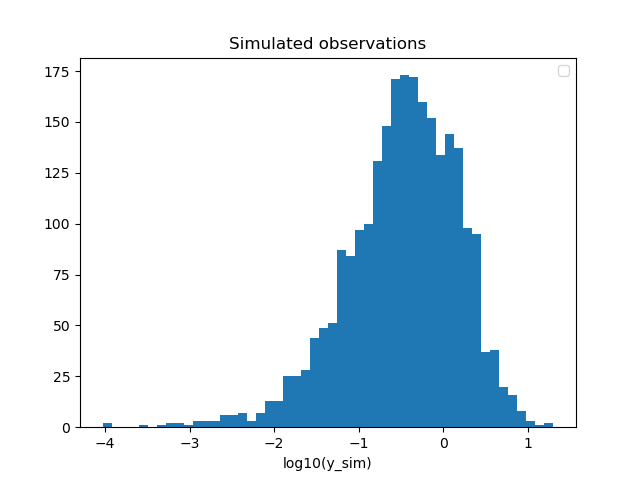
\includegraphics[width=0.5\linewidth]{../plots/original_simulated_observation.png}
	\caption{Distribution of the simulated observation using the yearly averaged emissions at all times.}
	\label{fig: y-histogram baseline}
\end{figure}


In order to quantify the performance of the simulations, we define some metrics. First of all, the fraction of the simulated observations which lie within a factor $2$ of the actual observations. In the ideal case, all simulated observations $\hat{y}$ would be exactly the same as the observed ones $y$. This metric allows for some small scaling factor as error.
\begin{equation}
	\text{FAC2}:=P(0.5\leq\hat{y}/y\leq 2)
\end{equation}

The previous metric only takes into account the simulated observations within a small area. Therefore it cannot tell us whether some general bias is present. To investigate this, we use the geometric mean bias. The more biased the ratio is, the further this value will lie from $1$. This is because it defines some mean ratio of actual observations and simulated ones.
%Nitpick Thomas: err, I did not actually check the formulae for the metrics closely during the week. It seems slightly weird taking the exponential, as we mostly care about the scalings (in log space). It might complicate the explanation: "needs to be close to 1 (in some logarithmic way)". Also, why do we have this minus sign in front?
\begin{equation}
	\text{GM}:=e^{-E(ln(\hat{y}/y))}
\end{equation}

\begin{figure}
	\centering
	\begin{minipage}{.48\textwidth}
		\centering
		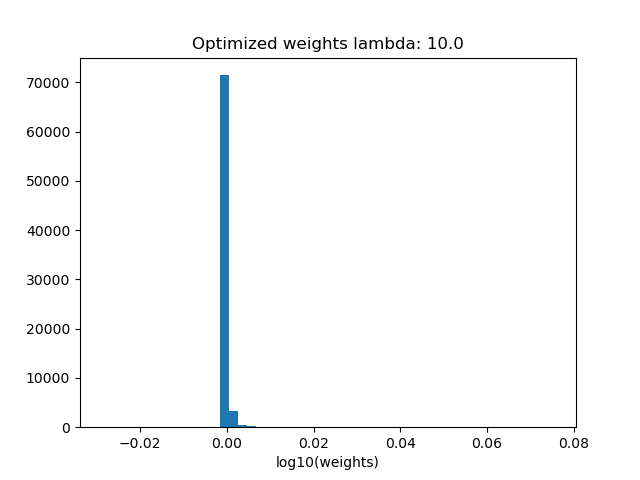
\includegraphics[width=0.9\linewidth]{../plots/hfun_weights_lambda10.png}
		\caption{Histogram of the optimized weights $W$, using a large regularization parameter $\lambda=10$.}
		\label{fig: optimized weights lambda=10}
	\end{minipage}\hfill
	\begin{minipage}{.48\textwidth}
		\centering
		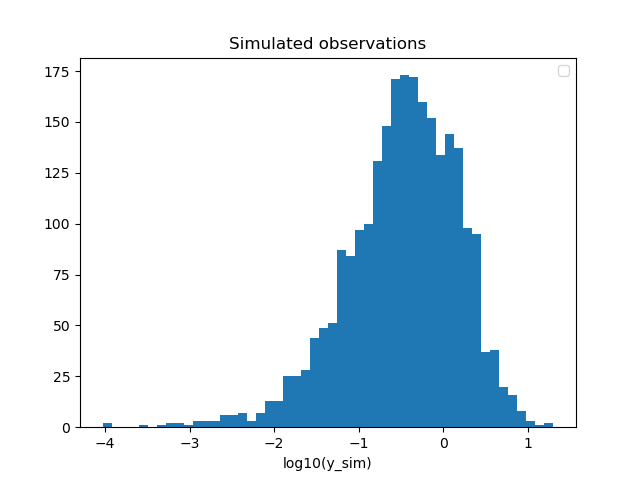
\includegraphics[width=0.9\linewidth]{../plots/hfun_simulated_observations_lambda10.png}
		\caption{Histogram of the ratio of simulated observations $\hat{y}/y$, using a large regularization parameter $\lambda=10$.}
		\label{fig: simulated observations lambda=10}
	\end{minipage}
\end{figure}

\begin{figure}
	\centering
	\begin{minipage}{.48\textwidth}
		\centering
		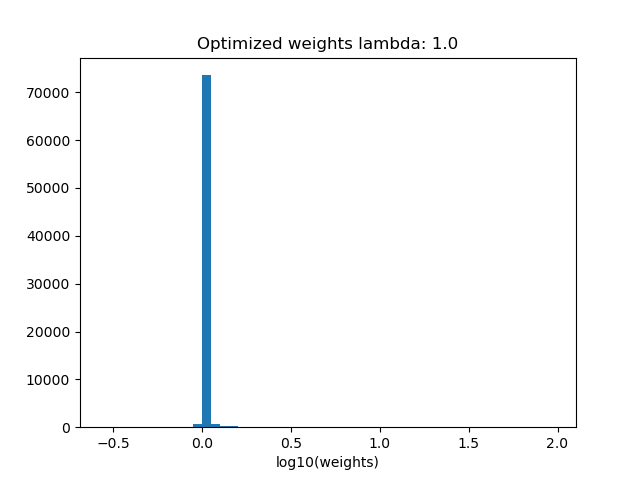
\includegraphics[width=0.9\linewidth]{../plots/hfun_weights_lambda1.png}
		\caption{Histogram of the optimized weights $W$, using a medium regularization parameter $\lambda=1$.}
		\label{fig: optimized weights lambda=1}
	\end{minipage}\hfill
	\begin{minipage}{.48\textwidth}
		\centering
		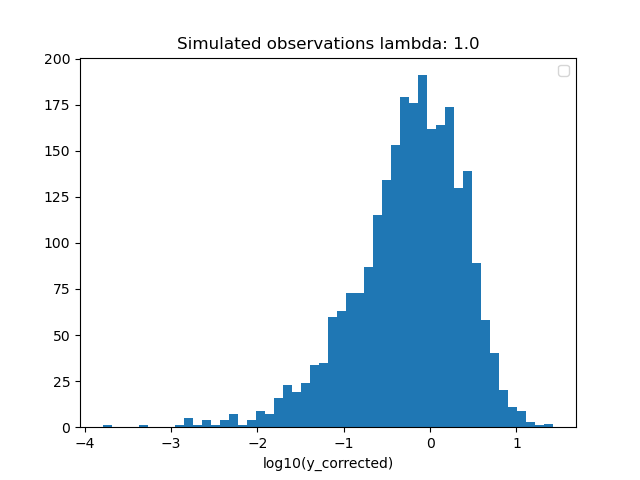
\includegraphics[width=0.9\linewidth]{../plots/hfun_simulated_observations_lambda1.png}
		\caption{Histogram of the ratio of simulated observations $\hat{y}/y$, using a medium regularization parameter $\lambda=1$.}
		\label{fig: simulated observations lambda=1}
	\end{minipage}
\end{figure}

\begin{figure}
	\centering
	\begin{minipage}{.48\textwidth}
		\centering
		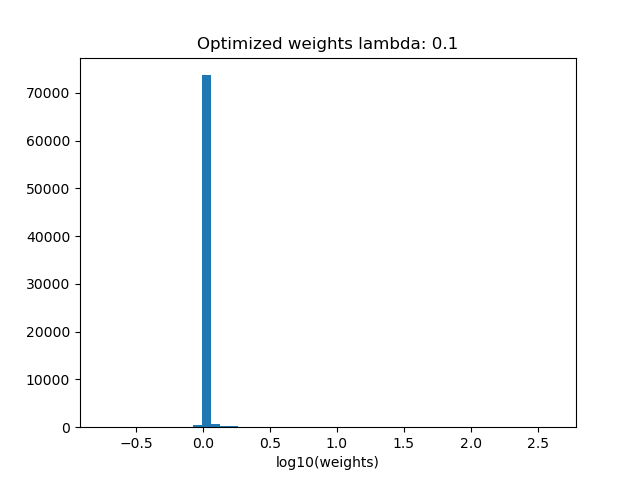
\includegraphics[width=0.9\linewidth]{../plots/hfun_weights_lambda01.png}
		\caption{Histogram of the optimized weights $W$, using a small regularization parameter $\lambda=0.1$.}
		\label{fig: optimized weights lambda=0.1}
	\end{minipage}\hfill
	\begin{minipage}{.48\textwidth}
		\centering
		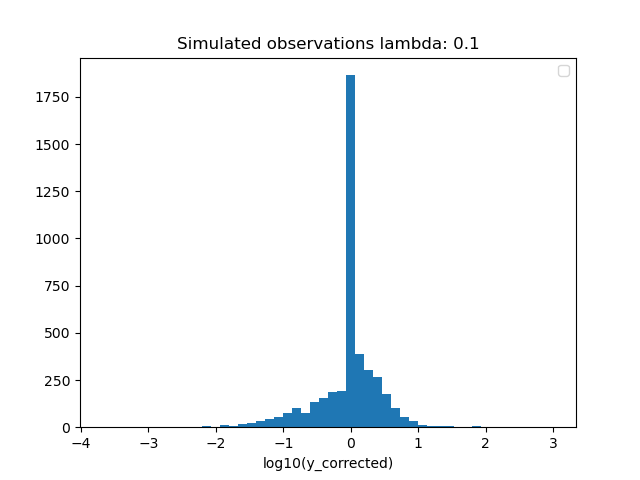
\includegraphics[width=0.9\linewidth]{../plots/hfun_simulated_observations_lambda01.png}
		\caption{Histogram of the ratio of simulated observations $\hat{y}/y$, using a small regularization parameter $\lambda=0.1$.}
		\label{fig: simulated observations lambda=0.1}
	\end{minipage}
\end{figure}

Starting with the results when using a high regularization parameter $\lambda=10$, we observe that the weights are nearly $1$ everywhere (see \cref{fig: optimized weights lambda=10}). This makes sense, as the cost function in this case heavily penalizes the weights for deviating from $1$. As a result, the histogram of simulated results (see \cref{fig: simulated observations lambda=10}) is nearly identical to the baseline. Lowering the regularization parameter $\lambda=1$, we find that the weights have more freedom to deviate from $1$ (see \cref{fig: optimized weights lambda=1}) and the bias on the ratio $\hat{y}/y$ decreases (see \cref{fig: simulated observations lambda=1}). This is a direct result of lowering the influence of the regularization term. Finally, lowering the regularization parameter $\lambda=0.1$ even further, the weights get even more freedom (see \cref{fig: optimized weights lambda=0.1}), while the ratio $\hat{y}/y$ finally seems to be centered around $1$. In \cref{table: evaluated metrics}, a summary of the metrics is found, evaluated at the different values for the regularization parameter. Summarized, we see the most major change in the geometric mean bias GM as the regularization parameter decreases. This might lead us to believe that the best result is obtained by choosing $\lambda$ as small as possible. However, a small value for $\lambda$ results in larger deviations from the mean emission; these can become greater than can what be expected in real life typical variation \cite{Ringbom2021,DeMeutter2016}. Thus a fine balance between the prediction error and the regularization condition is still needed.\\

To grant some intuition about the time dependence of the variability of the optimized emissions, the time series of the weights are plotted for different values of the regularization parameter (see \cref{fig: optimized weights timeseries lambda=10}, \cref{fig: optimized weights timeseries lambda=1}, \cref{fig: optimized weights timeseries lambda=0.1}). At first glance, all time series look erratic. Looking at the measured emission data in \cite{Ringbom2021}, the data is seemingly also erratic. This can support the claim that our optimized emissions could be realistic, however proper time series analysis is still needed to extract firm conclusions. At the same time, we see that all time series for the optimized weights look similar (ignoring the scale differences). This can be expected, as all optimized solutions try to fit the same data but are hindered in different amounts by their respective regularization parameter.


\begin{figure}
	\centering
	\begin{minipage}{.31\textwidth}
		\centering
		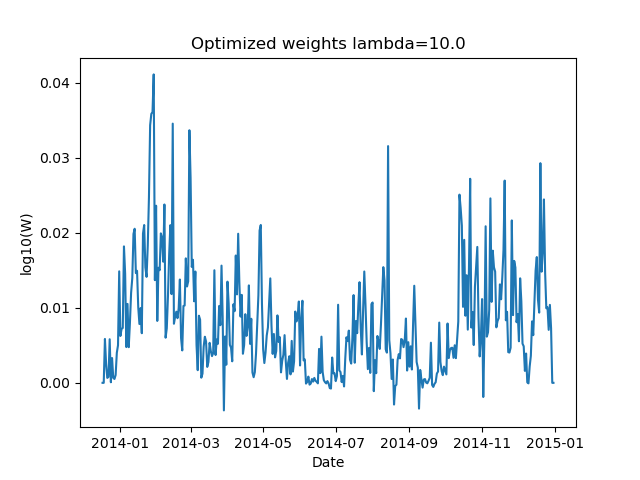
\includegraphics[width=\linewidth]{../plots/Optimized_weights_timeseries_lambda10.png}
		\caption{Time series of the optimized weights $W$, using a large regularization parameter $\lambda=10$.}
		\label{fig: optimized weights timeseries lambda=10}
	\end{minipage}\hfill
	\begin{minipage}{.31\textwidth}
		\centering
		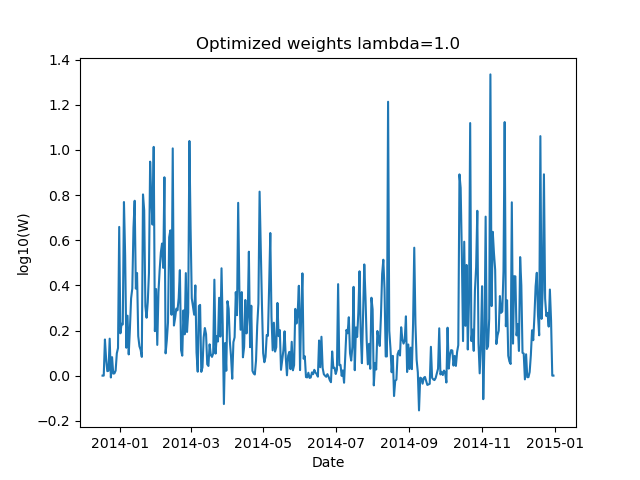
\includegraphics[width=\linewidth]{../plots/Optimized_weights_timeseries_lambda1.png}
		\caption{Time series of the optimized weights $W$, using a medium regularization parameter $\lambda=1$.}
		\label{fig: optimized weights timeseries lambda=1}
	\end{minipage}\hfill
	\begin{minipage}{.31\textwidth}
	\centering
	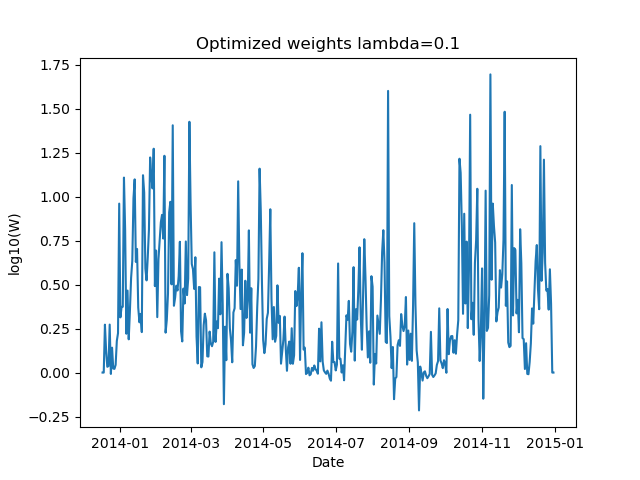
\includegraphics[width=\linewidth]{../plots/Optimized_weights_timeseries_lambda01.png}
	\caption{Time series of the optimized weights $W$, using a small regularization parameter $\lambda=0.1$.}
	\label{fig: optimized weights timeseries lambda=0.1}
	\end{minipage}
\end{figure}

\begin{table}
	\centering
	\caption{Metrics applied to the simulated observations in case of different regularization parameters $\lambda$.}\label{table: evaluated metrics}
\begin{tabular}{|l||c|c|}
	\hline
	&FAC2&GM\\\hline
	baseline&$31.7\%$&3.050\\\hline
	$\lambda=10$&$32.2\%$&2.984\\\hline	
	$\lambda=1$&$40.5\%$&1.776\\\hline	
	$\lambda=0.1$&$40.8\%$&1.216\\\hline
\end{tabular}
\end{table}

\section{Further work}
\label{sec: further work}
\begin{itemize}
    \item Standard software libraries support optimisation with constraints. This is an alternative to regularisation and may be more interpretable.
    Suppose that the number of components in $\tilde{x}$ is $m T$ (where $m$ is the number of sources and $T$ is the number of days).
    If we want to bound the average of $(\log w_{ij})^2$ by some value $\delta^2$, then we have the constrained optimisation problem
    \begin{align*}
        \min\quad & \frac{1}{2} \norm{\log h.(\hat{y})}^2 \\
        \text{s.t.}\quad & \frac{1}{mT} \norm{\log W}^2 \le \delta^2
    \end{align*} 
    which can be solved using similar ideas as those developed above. The prototypical constrained optimisation method (such as an active set method) would iterate towards a critical point of the Lagrangian
    $$
    \mathcal{L}(W, \lambda) = \frac{1}{2} \norm{\log h.(\hat{y})}^2 + \lambda\left(\frac{1}{mT} \norm{\log W}^2 - \delta^2\right)
    $$
    in which case the computational cost would be comparable to optimising \cref{eq: cost function regularised}. A more detailed explanation of constrained optimisation and the Lagrangian is found in \cite{Nocedal2006}.
    \item Currently, there is no constraint saying that, for every emission source $j$, the geometric mean of the emission should be the reported average $x_j$. This can be enforced with a constraint like $\prod_{t} w_{jt} = 1$ for all sources $j=1,\dots,m$. With the parametrisation $w = e^v$, this is equivalent to the linear constraint $\sum_{t} v_{jt} = 0$. Since this is a linear constraint, it can be handled relatively easily.
    \item For certain emission sources in certain periods, there is an expected correlation between the emission at time $t$ and at time $t + 1, t + 2, \dots$. We can add a constraint on the autocorrelation.
    \item Time-correlation could be measured by parameterising the model as follows: 
    \begin{align*}
        x_1^{2 \text{ Jan } 2014} &= \alpha_1^{(1)} x_1^{1 \text{ Jan } 2014} \\
        x_1^{3 \text{ Jan} 2014} &= \alpha_2^{(1)} x_1^{2 \text{ Jan } 2014} \\
        &\vdots
    \end{align*}
    with a constraint like $\alpha_{\min} \le \prod_{t=1}^T \alpha_t^{(j)} \le \alpha_{\max}$ for all $T$ and all $j = 1,\dots,m$. However, this would be difficult to implement. In addition, the complexity of inequality constrained optimisation can be combinatorial in the number of constraints if an active set method is used \cite{Nocedal2006}.

    \item For the sake of simplicity, the current implementation does not store $M_{shift}$ in memory in a data structure for large and sparse matrices. This could be changed to improve memory use and/or computation time.
    
    \item Other numerical optimisation algorithms may be more efficient or have better convergence properties. For instance, the Gauss-Newton and Levenberg-Marquardt methods are specifically designed for optimising the squared norm of a vector-valued function, but may require a large amount of memory \cite[Section 10.3]{Nocedal2006}.
    
\end{itemize}
    
\section{Anomaly detection}


One of the main challenges of applying traditional anomaly detection methods on the time-series data of an observation station, is accommodating for weather. Winds will change the course of an emission, causing different observation stations to pick up their signature. Therefore treating stations individually to try to learn their normal behavior would not lead to fruitful results. At the same time, it is also difficult to train more complex models that handle data collectively from all stations, since there is not enough historic data, and only a few observation stations are actively collecting data throughout the entire year.\\

For these reasons, working with the emission sources directly is more appealing. Correcting the emission data in the previous chapters allows us to obtain a better ground truth for the variation of the emissions over the course of the year. The resulting individual time-series data should show a few characteristics that arise from the nature of these sources:
\begin{itemize}
    \item For power plants, a long-term baseline variation corresponding to yearly electricity demand, which should vary consistently given that our readings are all in the northern hemisphere.
    \item For medical isotope production facilities, a short term periodic trend corresponding to the working days of the week.  
\end{itemize}  

After adjusting for the yearly trend, the eventual solution should include two components. The first which will segment the time-series into pieces with distinct behavior or features, for example using shapelets \cite{10.1145/2623330.2623613}\cite{10.1007/978-3-030-39098-3_7} or change point detection algorithms \cite{TRUONG2020107299}. The second part is to train anomaly detection models or classifiers, that distinguish between segments of normal and abnormal behavior. The state of the art methods use 1D convolution neural networks \cite{KIRANYAZ2021107398} or bayesian probabilistic models \cite{https://doi.org/10.48550/arxiv.1902.08627}. Finally, synthetic emission data should be simulated in order to evaluate these methods, since data for nuclear tests is rare if not inexistent.

    
\printbibliography

\end{document}

